\chapter{Mercoledì 20/05/2020}
\section{Organizzazione fisica e gestione della memoria}
\subsection{Memoria principale, memoria secondaria e gestione dei buffer}
Il DBMS è una \emph{scatola nera}. Non è strettamente necessario conoscere la sua struttura per poterne comprendere il funzionamento, ma in certe circostanze può essere utile.
\paragraph{Ricordiamo} Un DBMS gestisce collezioni di dati grandi, persistenti, condivisi. Garantisce affidabilità e privatezza. Deve essere anche efficiente (ridurre i tempi e sfruttare al meglio le risorse) ed efficace (rendere produttiva l'attività di ogni singolo utente).
\paragraph{Grandezza e persistenza} Il fatto che i dati siano grandi e persistenti richiede una gestione sofisticata della memoria secondaria. Gli utenti vedono il modello logico, ma le strutture che si celano dietro devono essere gestite efficientemente. Adotteremo delle strutture dati opportune.
\paragraph{Affidabilità} La base di dati deve essere preservata, come già detto, anche in caso di malfunzionamento. L'affidabilità è impegnativa per via di aggiornamenti frequenti e per la gestione del buffer.
\paragraph{Condivisione} Una base di dati è una risorsa condivisa fra più applicazione. Sono previsti meccanismi di autorizzazione e il cosiddetto controllo di concorrenza per gestire attività diverse e multi-utente su dati condivisi.
\begin{center}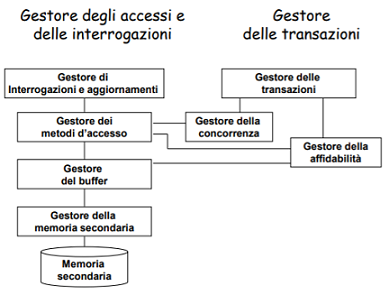
\includegraphics{images/174.PNG}\end{center}
\paragraph{Tecnologie presenti}
\begin{itemize}
	\item Gestione della memoria secondaria e del buffer
	\item Organizzazione fisica dei dati
	\item Ottimizzazione delle interrogazioni (sfruttando il concetto di equivalenza e sfruttando dati a nostra disposizione per determinare la miglior forma di ottimizzazione)
\end{itemize}
\begin{center}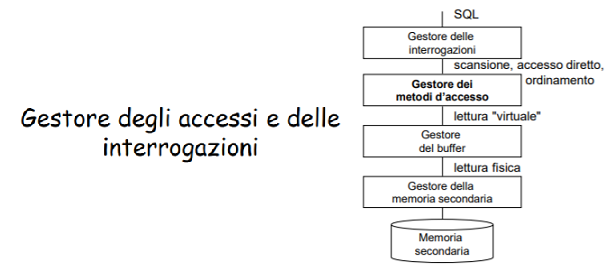
\includegraphics{images/175.PNG}\end{center}
\paragraph{File system e DBMS}
\begin{itemize}
	\item Il file system è il componente del sistema operativo che gestisce la memoria secondaria.
	\item I DBMS ne utilizzano le funzionalità per creare ed eliminare file e per leggere/scrivere singoli blocchi o sequenze di blocchi contigui. 
	\item Il DBMS gestisce i file allocati come se fossero un unico grande spazio di memoria secondaria e costruisce, in tale spazio, le strutture fisiche con cui implementa le relazioni.
\end{itemize}
\paragraph{Ricordare} Il programma non può entrare in contatto con la memoria secondaria ma solo con quella principale. Abbiamo il buffer che permette un'interazione fra memoria principale e secondaria, limitando il più possibile gli accessi alla secondaria.
\paragraph{Gerarchia di memoria}Abbiamo una serie di memoria, ciascuna con tecnologie e costi diversi. Si distinguono le memoria primarie, volatili, dalle memorie secondarie e terziarie, permanenti. Ovviamente il costo di mantenimento di una memoria di tipo permanente è più elevato.
\begin{center}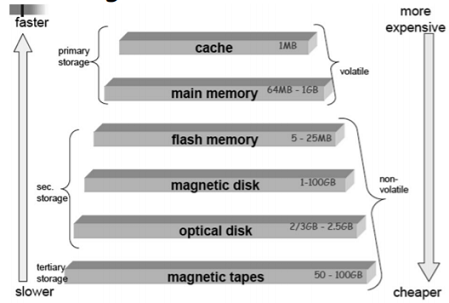
\includegraphics{images/176.PNG}\end{center}
Nell'accesso a memoria secondaria abbiano una testina che deve raggiungere il punto opportuno. Si considerano i seguenti tempi:
\begin{itemize}
	\item tempo di posizionamento della testina (10-50ms)
	\item tempo di latenza (5-10ms)
	\item tempo di trasferimento (1-2ms)
\end{itemize}
In media non meno di 10ms. Si osserva che l'accesso a memoria secondaria è quattro o più ordini di grandezza maggiore di quello per operazioni in memoria principale. Segue che il costo delle operazioni dipende moltissimo dal numero di accessi in memoria secondaria.
\paragraph{Organizzazione delle memorie} Ricordiamo che le memorie secondarie sono organizzate in blocchi di lunghezza fissa, mentre la memoria principale è organizzata in pagine. Nella memoria secondaria  le uniche operazioni possibili sono quelle di lettura e scrittura dei dati di un blocco: in riferimento alla latenza (citata prima) si osserva che l'accesso a blocchi vicini è molto meno costoso (latenza a 0).
\subsection{Buffer} Il buffer è un'area di memoria centrale gestita dal DBMS e condivisa fra le transazioni. Risulta organizzato in pagine di dimensioni pari o multiple di quelle dei blocchi di memoria secondaria (ricordiamoci che siamo in memoria principale). Il caricamento di una pagina del buffer equivale a un'operazione di lettura in memoria secondaria, mentre salvare una pagina equivale a un'operazione di scrittura.
\paragraph{Buffer manager} Questo, oltre al buffer, si occupa di una directory che per ogni pagina mantiene il file fisico e il numero del blocco, e due variabili di stato: 
\begin{itemize}
	\item un contatore che indica quanti programmi utilizzano la pagina; 
	\item un bit che indica se la pagina è \emph{sporca}, cioè se è stata modificata. 
\end{itemize}
Si considera:
\begin{itemize}
	\item l'alta probabilità di dover riutilizzare i dati attualmente in uso
	\item la legge di Pareto: l'80\% delle operazioni utilizza sempre lo stesso 20\% dei dati.
\end{itemize}
Il buffer si occupa di:
\begin{itemize}
	\item di ricevere richieste di lettura e scrittura dalle transazioni
	\item di eseguire queste operazioni accedendo alla memoria secondaria solo quando indispensabile
\end{itemize}
Ricordiamo, a proposito di queste richieste, le primitive:
\begin{itemize}
	\item fix: richiesta di pagina. Richiedo una lettura solo se la pagina non è nel buffer. Incrementa il contatore associato alla pagina offerta dal buffer manager
	\item setDirty: comunica che la pagina è stata modificata
	\item unfix: indica che la transazione ha concluso l'utilizzo della pagina (decremento il contatore associato alla pagina)
	\item force: trasferisco una pagina in memoria secondaria (su richiesta del gestore dell'affidabilità, non del gestore degli accessi)
\end{itemize}
\paragraph{Esecuzione della fix} 
\begin{itemize}
	\item cerco la pagina nel buffer
	\item se la trovo restituisco l'indirizzo
	\item se non la trovo cerco una pagina libera nel buffer (contatore $0$):
	\begin{itemize}
		\item se la trovo inserisco i dati letti dalla memoria secondaria e ne restituisco l'indirizzo
		\item se non la trovo ho due opzioni:
		\begin{itemize}
			\item seleziono una pagina \emph{vittima} occupata dal buffer, scrivo i dati di questa in memoria secondaria, effettuo le letture in memoria secondaria e restituisco l'indirizzo
			\item pongo in attesa l'operazione
		\end{itemize}
	\end{itemize}
\end{itemize}
\paragraph{Scopo della gestione del buffer} Vogliamo ridurre il numero di accessi alla memoria secondaria:
\begin{itemize}
	\item in caso di lettura, se la pagina è già presente nel buffer non c'è bisogno di accedere alla memoria secondaria
	\item in caso di scrittura, il gestore del buffer può decidere di differire la scrittura fisica in modo da accorparla ad altre scritture.
\end{itemize}
\paragraph{Scrittura in memoria secondaria} Il buffer manager può far partire le scritture in due contesti diversi:
\begin{itemize}
	\item in modo sincrono quando è richiesto esplicitamente con una force
	\item in modo asincrono, cioè quando lo ritiene opportono. Si possono anticipare o posticipare scritture per coordinarle e/o sfruttare la disponibilità dei dispositivi.
\end{itemize}
\subsection{Gestione delle tuple nelle pagine}
\paragraph{Tuple e blocchi}
\begin{itemize}
	\item Il file system ha i suoi file: questi sono logicamente organizzati in record. 
	\item I record sono mappati nei blocchi di memoria secondaria. 
	\item Le tuple di una relazione (record di file) stanno in blocchi contigui. A volte in un blocco ci sono tuple di relazioni diverse ma correlate (i JOIN  sono favoriti)
	\item I blocchi (componenti fisici di un file) e le tuple o record (componenti logici di una relazione) hanno dimensioni in generale diverse:
	\begin{itemize}
		\item la dimensione del blocco dipende dal file system
		\item la dimensione del record dipende dalle esigenze dell'applicazione e può anche variare nell'ambito di un file.
	\end{itemize}
\end{itemize}
\paragraph{Organizzazione delle tuple}
Ho varie alternative possibili. Solitamente inseriamo le tuple in modo sequenziale nei file. Inoltre:
\begin{itemize}
	\item se la lunghezza delle tuple è fissa, la struttura può essere semplificata
	\item alcuni sistemi possono spezzare le tuple su più blocchi (tuple grandi, cosa difficile da gestire)
\end{itemize}
\paragraph{Fattore di blocco} Attraverso il fattore di blocco stabilisco quanti record posso porre in un blocco.
\begin{itemize}
	\item $L_R$: dimensione di un record (per semplicità costante nel file: record a lunghezza fissa)
	\item $L_B$: dimensione di un blocco
	\item se $L_B>L_R$ possiamo avere più record in un blocco
	\begin{center}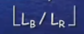
\includegraphics{images/177.PNG}\end{center}
	\item lo spazio residuo può essere utilizzato per record \emph{spanned} o non utilizzato.
\end{itemize}
\paragraph{Esercizio} Calcolare il fattore di blocco e il numero di blocchi occupati da una relazione contenente $T=500000$ tuple di lunghezza fissa pari a $L=100$ byte in  un sistema con blocchi di dimensione pari a $B=1$ kilobyte. Risolviamo così:
\begin{itemize}
	\item $N_B=D_T/B$
	\item $D_T=T*L$
	\item $F_B=B/L$
	\item $F_B=1024/100$
\end{itemize}
\paragraph{Operazioni sulla pagina} 
\begin{itemize}
	\item Inserimento/Modifica di una tupla (la cosa può richiedere allocazione di ulteriore spazio)
	\item Cancellazione
	\item Accesso ad una tupla o ad un campo di una tupla
\end{itemize}
\subsection{Strutture per l'organizzazione di file}
\paragraph{Definizioni}
\begin{itemize}
	\item Le tuple organizzate all'interno dei blocchi dei file costituiscono le \textbf{strutture primarie}, cioè quelle che contengono propriamente i dati. Le principali sono
	\begin{itemize}
		\item strutture sequenziali (seriali / ordinate / ad array)
		\item strutture ad accesso calcolato (hash)
		\item strutture non sequenziali ad albero
	\end{itemize}
	\item Esistono anche blocchi contenenti \textbf{strutture secondarie}, che sono quelle che favoriscono l'accesso ai dati senza contenerli (in un certo senso sono dei puntatori ai dati).
\end{itemize}
\subsubsection{Strutture primarie sequenziali} Una struttura primaria sequenziale può essere
\begin{itemize}
	\item \textbf{seriale} (detto anche \emph{heap}, miscuglio): ordinamento fisico ma non logico. Gli inserimenti vengono effettuati:
	\begin{itemize}
		\item in coda (gli elementi sono di fatto posti nell'ordine di inserimento)
		\item al posto di record cancellati (che ho precedentemente sostituito con una \emph{marca} che mi segnala la cancellazione)
	\end{itemize}
	L'eliminazione, ma anche la sostituzione di una tupla con un'altra di dimensione minore, comportano uno spreco di spazio e un conseguente aumento del numero di blocchi utilizzati: segue la necessità di svolgere riorganizzazioni periodiche. Una ricerca è di tipo sequenziale: segue una complessità lineare e la necessità di scorrere, nel caso peggiore, tutto il file.
	\item \textbf{ordinata}: ordinamento fisico delle tuple coerente con quello di un campo detto chiave (per esempio, data una lista di studenti universitari, la matricola)
	\begin{itemize}
		\item Sono possibili ricerche binarie
	\end{itemize}
	Le riorganizzazioni periodiche sono necessarie anche in questo tipo di organizzazione. Si ha un'ulteriore problema: dobbiamo mantenere l'ordinamento a seguito di un qualunque cambiamento. Ciò rende le riorganizzazioni decisamente più importanti e complesse.
	\item \textbf{array}: le tuple hanno stessa dimensione, all'interno di uno o più blocchi contigui abbiamo una serie di posizioni identificate da indici. 
	\begin{itemize}
		\item Il caricamento iniziale delle informazioni avviene mediante incremento di un contatore e inserimento nelle varie posizioni
		\item La cancellazione lascia spazi vuoti
		\item Gli inserimenti possono essere effettuati solo in posizioni vuote o in fondo al file. 
	\end{itemize}
	Generalmente questa struttura non è quasi mai utilizzata nei DBMS. 
\end{itemize}
\subsubsection{Strutture primarie ad accesso calcolato}
Questa struttura, detta anche \emph{hash}, sfrutta le proprietà tipiche dell'organizzazione sequenziale ad array anche in circostanze in cui l'array non risulta immediatamente applicabile. L'array, normalmente, è ottimo, per organizzare insiemi di record che hanno come \emph{campo chiave} valori consecutivi (esempio numero di matricole da 1 a 10000): questa cosa, in moltissime situazioni, non è possibile.
\begin{itemize}
	\item i file hash permettono un accesso diretto molto efficiente. 
	\item Ricordiamo che la funzione hash:
	\begin{itemize}
		\item associa ad ogni valore della chiave un "indirizzo", in uno spazio di
		dimensione leggermente superiore rispetto a quello
		strettamente necessario
		\item poiché il numero di possibili chiavi è molto maggiore del numero
		di possibili indirizzi, la funzione non può essere iniettiva e quindi
		esiste la possibilità di collisioni (chiavi diverse che corrispondono
		allo stesso indirizzo) 
		\item le buone funzioni hash distribuiscono in modo causale e uniforme,
		riducendo le probabilità di collisione (che si riduce aumentando
		lo spazio ridondante) 
	\end{itemize}
\end{itemize}
\paragraph{Come risolvo le collisioni?} Esistono varie tecniche:
\begin{itemize}
	\item Occupare le posizioni successive
	\item Ricorrere a tabelle/catene di overflow (gestita in forma collegata)
	\item Adottare funzioni hash alternative
\end{itemize}
Osserviamo che:
\begin{itemize}
	\item le collisioni sono quasi sempre presenti (tenendo conto che non possiamo avere funzioni iniettive nella maggior parte dei casi)
	\item le collisioni multiple hanno probabilità che decresce al crescere della molteplicità
	\item la molteplicità media delle collisioni è molto bassa
\end{itemize}
\paragraph{Hash su file} Ricordiamo l'organizzazione di un file: esso è diviso in blocchi, e questi a loro volta presentano all'interno delle tuple. La funzione hash restituisce un indice rappresentante il blocco all'interno del quale è presente la tupla incriminata. Questo ci permette di ammortizzare le probabilità di collisione
\begin{itemize}
	\item In caso di conflitto il record è memorizzato nello stesso blocco dove sono presenti altre tuple
	\item Quando lo spazio di un blocco è esaurito viene allocato un ulteriore blocco, collegamento al precedente, e il record viene posto al suo interno. Questa tecnica è detta \emph{catena di overflow}.
	\item Segue che per una parte di tuple, associate a un certo indice, sarà necessario un solo accesso a blocco. Per questa tupla, appena aggiunta, invece, serviranno due accessi!
\end{itemize}
\paragraph{Esempio di esercizio}
\begin{itemize}
	\item Prendiamo la seguente tavola hash (con collisioni) e facciamo delle analisi relative all'\emph{hash su file}
	\begin{center}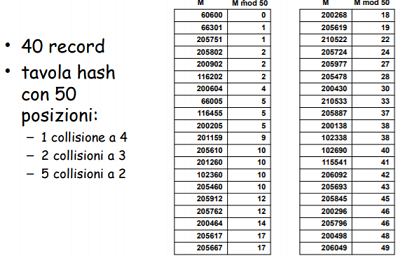
\includegraphics{images/178.PNG}\end{center}
	\item Consideriamo:
	\begin{itemize}
		\item $T$ il numero di tuple previsto per il file
		\item $F$ il fattore di blocco
		\item $f$ il fattore di riempimento (la frazione dello spazio fisico disponibile mediamente utilizzata)
	\end{itemize}
	\item Svolgiamo il seguente calcolo per trovare il numero di blocchi utilizzato
	\[B=\frac{T}{f \times F}=\frac{40}{\frac{4}{5} \times 10} = 5\]
	\item Abbiamo 5 blocchi con 10 posizioni ciascuno!
	\item Prendiamo la seguente figura, che contiene gli stessi dati della precedente tavola hash
	\begin{center}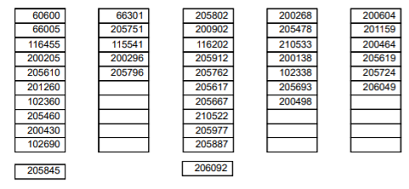
\includegraphics{images/230.PNG}\end{center}
	Complessivamente abbiamo $30$ chiavi: per raggiungere due chiavi è necessario l'accesso a due blocchi, uno solo per le rimanenti $28$.
\end{itemize}
\subsubsection{Strutture ad albero (non sequenziali, dette \emph{indici})} Le strutture ad albero, come quelle \emph{hash}, favoriscono l'accesso ai dati in base al valore di uno o più campi. Sono consentiti accessi
\begin{itemize}
	\item puntuali
	\item corrispondenti a intervalli di valori
\end{itemize}
L'organizzazione ad albero, come vedremo, può essere utilizzata per realizzare sia strutture primarie che secondarie.

\paragraph{Cosa intendiamo con indice?} Supponiamo di avere un file $f$ e un campo chiave (che può avere al suo interno più attributi): un \textbf{indice secondario} consiste in un altro file dove ciascun record è logicamente composto da due campi:
\begin{itemize}
	\item uno contenente il valore del campo chiave
	\item uno contenente l'indirizzo o gli indirizzi fisici dei record del file $f$ che hanno quel valore di chiave
\end{itemize}
Un esempio per capire in cosa effettivamente consiste un indice secondario è l'indice analitico presenti in fondo a certi libri: ho un ordine alfabetico dei termini presenti e le pagine dove sono presenti tali termini. Un indice si dice \textbf{indice primario} se l'ordinamento è lo stesso della struttura dati o se contiene al suo interno i dati: in questo caso non garantisco solo un accesso in base a un campo chiave, ma contengo anche i record fisici necessari per memorizzare i dati. Un esempio per comprendere l'indice primario è l'indice generico presente in ogni libro: ho le sezioni e il numero delle pagine dove queste sono posizionate.
\subparagraph{File} Un file può avere un solo indice primario (questo non è presente solo quando l'organizzazione primaria è hash oppure sequenziale) e più indici secondari.
\paragraph{Puntatori in un indice} I puntatori di un indice reindirizzano
\begin{itemize}
	\item al blocco dove è presente la tupla, o
	\item alla tupla stessa.
\end{itemize}
il tempo per effettuare la ricerca di una tupla all'interno di un blocco è trascurabile. Questo ci permette di limitare, in certi casi, il numero di puntatori per blocco: potrei puntare alla tupla contenente valore della chiave minore o maggiore.
\paragraph{Indici densi e sparsi} Consideriamo gli indici con puntatori a tuple. Essi saranno detti:
\begin{itemize}
	\item \textbf{densi}, se tutte le tuple dei vari blocchi sono puntate da elementi dell'indice (solitamente quando adottiamo un'ordinamento diverso da quello fisico e quindi non è più possibile garantire la presenza di una tupla all'interno di un blocco).
	\item \textbf{sparsi}, se non tutte le tuple sono puntate (solitamente quando seguiamo l'ordinamento fisico, quindi puntando a una certa tupla di un blocco - rappresentante un valore di riferimento - sono certo che ciò che sto cercando sarà all'interno di quella tupla)
\end{itemize}
Gli indici secondari sono per forza densi, poichè basati su criteri di ordinamento diversi da quello fisico. L'indice primario può essere sparso.
\paragraph{Ricerche} Il fatto di avere un ordinamento permette di svolgere ricerche binarie con complessità logaritmica. Sono possibili anche ricerche basate su intervalli e scansioni sequenziali ordinate (cose inefficienti sulle strutture hash).
\paragraph{Caratteristiche degli indici}
\begin{itemize}
	\item Accesso diretto ed efficiente sulla chiave
	\item Modifiche della chiave, inserimenti, eliminazioni inefficienti (come nei file ordinati). Possiamo adottare le seguenti tecniche per migliorare la situazione:
	\begin{itemize}
		\item file o blocchi di overflow
		\item marcatura per le eliminazioni 
		\item riempimento parziale
		\item blocchi collegati (non contigui) 
		\item riorganizzazioni periodiche
	\end{itemize}
\end{itemize}
Segue una scarsa flessibilità in presenza di elevata dinamicità.
\paragraph{Indici multilivello}
\begin{itemize}
	\item Gli indici sono file essi stessi e quindi ha senso costruire indici sugli indici, per evitare di fare ricerche fra blocchi diversi 
	\item Possono esistere più livelli fino ad avere il livello più alto con un solo blocco; i livelli sono di solito abbastanza pochi, perché
	\begin{itemize}
		\item ogni nodo (al di fuori delle foglie) ha un numero di discendenti abbastanza elevato, dipendente dall'ampiezza della pagina.
		\item l'indice è ordinato, quindi l'indice sull'indice è sparso 
		\item i record dell'indice sono piccoli
	\end{itemize}
\end{itemize}
Sfruttando questi concetti andiamo a costruire degli alberi dove ciascun nodo consiste in un file, quindi in un indice!
\begin{center}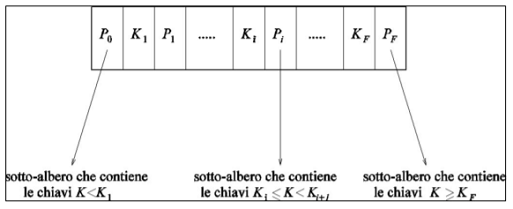
\includegraphics{images/229.PNG}\end{center}
\paragraph{Indici e alberi binari}
\begin{itemize}
	\item Gli indici utilizzati dai DBMS sono in generale
	\begin{itemize}
		\item indici dinamici multilivello 
		\item Vengono memorizzati e gestiti come B-tree (intuitivamente: alberi di ricerca bilanciati): Alberi binari di ricerca, Alberi n-ari di ricerca, Alberi n-ari di ricerca bilanciati
	\end{itemize}
\end{itemize}
Si ricorre ad alberi generici di ordine $P$ (dove ciascun nodo presenta fino a $P$ figli e $P-1$ etichette). Questi alberi saranno tenuti bilanciati nel tempo grazie a:
\begin{itemize}
	\item Riempimento parziale (mediamente 70\%) 
	\item Riorganizzazioni (locali) in caso di sbilanciamento
\end{itemize}
Si distingue una versione B-tree da una B+-tree: 
\begin{itemize}
	\item nel B+-tree a le foglie costituiscono una lista e sono collegate fra di loro
	\item nel B-tree possiamo avere, in nodi intermedi, puntatori diretti ai dati. 
\end{itemize}
\begin{multicols}{2}
	\begin{center}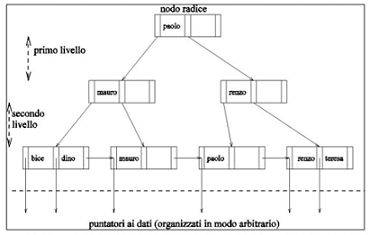
\includegraphics{images/181.PNG}\end{center}
	\begin{center}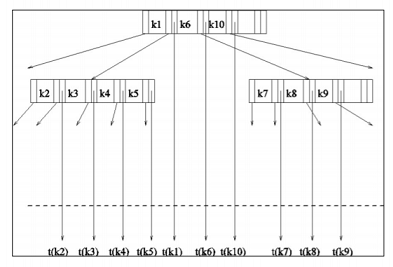
\includegraphics{images/182.PNG}\end{center}
\end{multicols}
Entrambi gli alberi sono molto efficienti: la forma preferita è la B+-tree in quanto permette di svolgere ricerche basate su un intervallo di valori. Con le foglie collegate posso effettuare selezioni basate su un intervallo di valori: individuo il primo valore dell'intervallo e poi effettuo una scansione sequenziale per trovare i valori maggiori rispetto a questo.
\paragraph{Definizione degli indici SQL}
Non è standard ma presente in forma simile nei vari DBMS
\begin{itemize}
	\item \begin{verbatim}create [unique] index IndexName on
		TableName(AttributeList)\end{verbatim}
	\item \begin{verbatim}drop index IndexName\end{verbatim}
\end{itemize}
\paragraph{Diapositive} Vedere attorno alla diapositiva 66 le strutture fisiche presenti in alcuni DBMS

\section{Esecuzione e ottimizzazione delle interrogazioni}
Riprendiamo un discorso iniziato con l'algebra relazionale. Abbiamo visto il \emph{query processor}, un modulo del DBMS nel quale avviene un processo di ottimizzazione basato su equivalenze (e sul catalogo, che contiene una serie di informazioni utili per l'esecuzione\footnote{Esempi di profili:\begin{itemize}\item cardinalità di ciascuna relazione \item dimensioni delle tuple e dei valori degli attributi \item numero di valori distinti degli attributi \item valore minimo e massimo di ciascun attributo\end{itemize}}). Le interrogazioni sono espresse ad alto livello (ricordare il concetto di indipendenza dei dati): insiemi di tuple, poca proceduralità.
\paragraph{Fase finale di ottimizzazione} Abbiamo lasciato in sospeso l'ultima delle tre fasi del \emph{query processor}. In questa abbiamo un'\textbf{ottimizzazione in base ai costi}: consideriamo il numero di trasferimenti in memoria da fare e stimiamo le dimensioni dei risultati intermedi. Nell'ottimizzazione dobbiamo tener conto anche
\begin{itemize}
	\item delle operazioni da eseguire (vedere paragrafo dopo)
	\item i dettagli del metodo (per esempio quale tipo di JOIN eseguire)
	\item ordine delle operazioni (ho un join di tre relazioni, da dove mi conviene partire?)
\end{itemize}
\paragraph{Implementazione degli operatori dell'AR} Le interrogazioni sono svolte mediante un linguaggio ad alto livello, cioè lontano dalla macchina. I DBMS implementano gli operatori dell'algebra relazionale per mezzo di operazioni di livello abbastanza basso. Abbiamo
\begin{itemize}
	\item \textbf{Operatori fondamentali}: accesso diretto e scansione
	\item \textbf{A livello più alto}: ordinamento
	\item \textbf{A livello ancora più alto}: JOIN, operazione più costosa (che coinvolge, ricordiamoci, il prodotto cartesiano).
\end{itemize}
\subsection{Accesso diretto}
Fare \emph{accesso diretto} significa ottenere, dato il valore di un campo, l'indirizzo del blocco in cui il record si trova. Ciò può essere fatto solo con strutture hash o indici. I tipi di accessi sono:
\begin{itemize}
	\item puntuali, del tipo $A_i=V$
	\item su intervallo, del tipo $V_1 \leq A_i \leq V_2$
\end{itemize}
Il primo tipo di accesso è efficiente in entrambe le strutture (in particolare in quelle hash), il secondo è efficiente solo negli accessi basati su indice. 
\paragraph{Interrogazioni} Nelle interrogazioni consideriamo predicati congiuntivi e disgiuntivi. Se si ha un solo predicato predicato valutabile conviene usare indice o hash. In caso contrario:
\begin{itemize}
	\item \textbf{predicati congiuntivi}\footnote{Cognome = 'Rossi' AND Nome = 'Maria'}: prima scelgo il più selettivo (quello che mi leva più tuple), dopo verifico gli altri scorrendo quanto salvato in memoria principale (cioè le tuple che rispettano il primo predicato). Nel caso hash pongo come argomento della funzione il cognome e verifico l'altra condizione.
	\item \textbf{predicati disgiuntivi}\footnote{Cognome = 'Rossi' OR Nome = 'Maria'}: se tutti i predicati sono valutabili utilizzo gli indici per ogni elemento. Sono convenienti, rispetto a una scansione, solo se molto selettivi. Bisogna fare attenzione anche ai duplicati. Il caso nel footnote è impossibile in hash.
\end{itemize}

\subsection{Scansione}
La scansione consiste in un'operazione di ricerca: è implementabile tramite un algoritmo di ricerca la cui complessità media, date $n$ tuple, è lineare. \textbf{I blocchi vengono trasferiti dalla memoria secondaria al buffer}.
\paragraph{Metodo alternativo} Un metodo alternativo è il ricorso agli indici. Inoltre, se 
\begin{itemize}
	\item le tuple \underline{sono ordinate}
	\item la selezione è fatta sull'attributo su cui la relazione è ordinata 
	\item i blocchi sono memorizzati in modo contiguo
\end{itemize}
allora possiamo ottenere un numero medio di trasferimenti logaritmico $\log_2 n$.

\subsection{Ordinamento}
La procedura di ordinamento è necessaria sia per ottenere risultati ordinati che per una corretta realizzazione delle proiezioni, con eliminazione dei duplicati. Risulta utile anche per implementare in modo efficiente operazioni come il JOIN, o il raggruppamento. Possiamo ottenere l'ordinamento con:
\begin{itemize}
	\item \textbf{quickSort}, se la relazione può essere posta tutta nel buffer;
	\item \textbf{mergeSort}, se la relazione non può essere posta tutta nel buffer e quindi dobbiamo lavorare su più frammenti.
\end{itemize}

\subsection{JOIN}
Il JOIN è l'operazione a più alto livello. Si hanno vari metodi:
\begin{itemize}
	\item Nested-loop (\textit{quello che si fa ad occhio} - cit)
	\item Merge scan
	\item Hash-based
\end{itemize}
\subsubsection{Nested-loop}
\paragraph{Algoritmo} Abbiamo una tabella, una \emph{interna} e una \emph{esterna}. Per ogni tupla della tabella esterna scandisco la tabella interna individuando le tuple che fanno JOIN.
\paragraph{Costo} 
\begin{itemize}
	\item Prendiamo le seguenti tabelle:
	\begin{itemize}
		\item Tabella $R$ con 10.000 record che occupano 400 blocchi
		\item Tabella $S$ con 5.000 record che occupano 100 blocchi.
	\end{itemize}
	\item Consideriamo $R$ esterna
	\item Prendiamo il caso peggiore: nel buffer si può inserire solo un record di $S$ alla volta, quindi devo effettuare innumerevoli accessi. Ottengo il seguente numero di trasferimenti
	\[N=10000*100+400\]
	Per ogni tupla della tabella $R$ scandisco tutti i blocchi della tabella $S$, portandoli ripetutamente in memoria. La tabella $R$ rimane nel buffer, quindi la porto in memoria principale soltanto una volta.
	\item Nel caso migliore, cioè quando tutta la tabella $S$ entra nel buffer, ottengo
	\[N=400+100\]
\end{itemize}

\subsubsection{Merge scan}
Questa tecnica si basa sull'ordinamento delle tabelle in base agli attributi di JOIN. L'algoritmo risulta molto efficiente quando le tabelle sono già ordinate o se sono presenti indici adeguati. 
\begin{itemize}
	\item Fondamentalmente abbiamo una scansione in parallelo delle due tabelle, come nella funzione \emph{merge} dell'algoritmo \emph{mergeSort}.
	\item Quando i valori dei due attributi coincidono ottengo una tupla appartenente al risultato. Il meccanismo fa sì che il risultato sia ordinato.
\end{itemize}
Il costo consiste nei trasferimenti in memoria ($N=br+bs$, ogni blocco è letto una volta soltanto assumendo che tutte le tuple per un dato valore di JOIN stiano insieme nel buffer) e nell'ordinamento (questo se le tabelle non sono già ordinate). L'algoritmo è utilizzato per il JOIN naturale o l'Equi-JOIN. 

\subsubsection{Hash-JOIN}
\begin{itemize}
	\item Utilizzo una funzione $h$ di hash sugli stessi attributi per memorizzare una copia di ciascuna delle due tabelle (difetto del metodo è un utilizzo maggiore di memoria) in memoria centrale
	\item La funzione $h$ comporta una partizione delle tabelle $R$ ed $S$ coinvolte: dati i valori del dominio di tali attributi ottengo come risultato lo stesso indice.
	\item L'indice identificherà una partizione di $R$ ed una di $S$: a quel punto mi basta effettuare dei semplici JOIN tra queste partizioni.
\end{itemize}
Questa tecnica è utile solo per JOIN-naturale ed Equi-JOIN, quest ultimo svolto in modo più efficiente se confrontato con il nested-loop.
\paragraph{Costo del metodo} 
\begin{itemize}
	\item Le relazioni $R$ ed $S$, per essere partizionate, devono essere portate in memoria centrale. Intanto individuiamo i seguenti trasferimenti
	\[2(br+bs)\]
	Due volte poichè dobbiamo svolgere un'operazione di lettura e una di scrittura
	\item Per ogni tupla $t_r$, in ogni partizione di $R$, si considera la tupla $t_s$ nella partizione corrispondente secondo la funzione hash, quindi si legge ciascuna partizione una volta. Seguono ulteriori trasferimenti
	\[(br+bs)\]
	\item Il costo complessivo dell'hash-JOIN sarà
	\[3(br+bs)\]
\end{itemize}
\pagebreak

\subsection{Misura del costo di una query}
Molti fattori contribuiscono al costo di una query, cioè il tempo necessario per avere la risposta:
\begin{itemize}
	\item L'accesso al disco, il tempo predominante calcolabile considerando:
	\begin{itemize}
		\item il numero di scansioni
		\item il numero di lettura
		\item il numero di scritture
	\end{itemize}
	\item il tempo di CPU
	\item il tempo di rete
\end{itemize}
Poniamo per semplicità il fattore $t$ unico come tempo per accedere a un blocco. 
\begin{itemize}
	\item Dobbiamo considerare, oltre al numero di trasferimenti, la memoria utilizzata per memorizzare i risultati intermedi. 
	\item Abbiamo ribadito come l'hash-JOIN necessiti di tabelle intermedie.
	\item Operazioni con più operandi devono essere eseguite uno step alla volta.
	\begin{itemize}
		\item \textbf{Congiunzione di condizioni}:
		\begin{itemize}
			\item Una congiunzione di operazioni di selezione può essere scomposta in una sequenza di selezioni semplici
			\[\sigma_{\theta1 \ni \theta2}(R)=\sigma_{\theta1}(\sigma_{\theta2}(R))\]
			\item Le operazioni di selezione sono commutative
			\[\sigma_{\theta1}(\sigma_{\theta2}(R))=\sigma_{\theta2}(\sigma_{\theta1}(R))\]
			\item L'ordine viene scelto in base alla dimensione del risultato intermedio.
		\end{itemize}
		\item \textbf{Ordine dei JOIN}
		\begin{itemize}
			\item L'ordine in cui si fanno i JOIN dipende dalla dimensione dei risultati intermedi
			\item Date le relazioni $R1, R2, R3$, sappiamo che vale la proprietà associativa
			\[(R1 \Join R2) \Join R3 = R1 \Join (R2 \Join R3)\]
			\item Se la dimensione di $R2 \Join R3$ è molto grande e quella di $R1 \Join R2$ è piccola, conviene eseguire i JOIN nel seguente ordine
			\[(R1 \Join R2) \Join R3\]
			in modo da dover memorizzare una relazione intermedia più piccola
		\end{itemize}
	\end{itemize}
\end{itemize}
\pagebreak
\paragraph{Processo di ottimizzazione}
Si costruisce un albero di decisione con le varie alternative, si valuta il costo di ciascun piano e si sceglie il piano di costo minore. L'ottimizzatore sceglie di solito una soluzione \emph{buona} non necessariamente una soluzione \emph{ottima}.
\begin{center}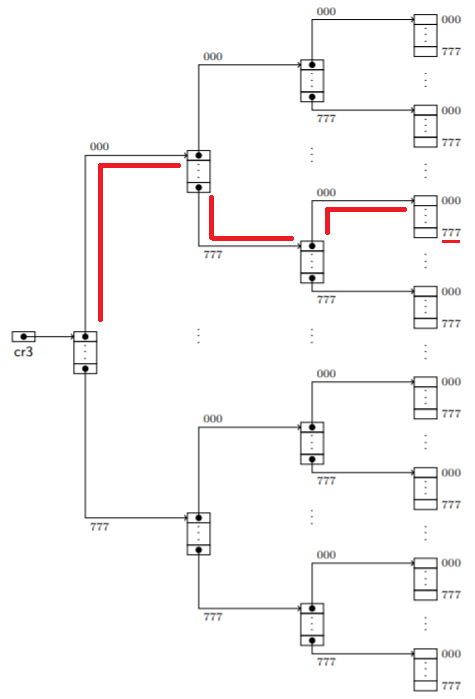
\includegraphics{images/232.PNG}\end{center}

\paragraph{Esercizio} Calcoliamo il piano di esecuzione migliore per la seguente interrogazione dal punto di viste della dimensione dei risultati intermedi
\[\pi_T(\sigma_{(C=D\,\lor\,C=B) \,\land \,A=X \,\land \,N=Y}(F \Join Ac \Join I)\]
Abbiamo le seguenti tabelle
\begin{Verbatim}[commandchars=+\[\]]
	F(+underline[Fid], Titolo, Anno, Categoria, ...)
	Ac(+underline[Aid], Nazionalità, ...)
	I(+underline[Fid, Aid],...)
\end{Verbatim}
E i seguenti dati:
\begin{itemize}
	\item Numero di tuple in $F$: $N(F)=30000$
	\item Numero di tuple in $A$: $N(A)=2000$
	\item Numero di tuple in $I$: $N(I)=600000$
	\item Numero di film distinti nelle interpretazioni: $N(Fid, I)=30000$
	\item Numero di attori distinti nelle interpretazioni: $N(Aid, I)=2000$
	\item Numero di nazionalità distinte tra gli attori: $N(Nazionalita, A)=4$
	\item Numero di categorie distinte tra i film: $N(Categoria, F)=5$
	\item Numero di anni distinti tra i film: $N(Anno, F)=20$
\end{itemize}
Procediamo
\begin{enumerate}
	\item Per prima cosa eseguiamo le ottimizzazioni sempre valide. Applicando \emph{push selections down} e \emph{push projections down} otteniamo
	\[\pi_T(\pi_{T,FId}(\sigma_{(C=D\,\lor\,C=B)\,\land\,A=X}(F)) \Join \pi_{AId}(\sigma_{N=Y}(Ac)) \Join \pi_{FId,AId}(I))\]
	\item Prendiamo $\pi_{T,FId}(\sigma_{(C=D\,\lor\,C=B)\,\land\,A=X}(F))$
	\begin{itemize}
		\item $\sigma_{(C=D\,\lor\,C=B)}(F)$
		\begin{itemize}
			\item Vogliamo stabilire che gli oggetti appartengono alla categoria $C$ o alla categoria $D$
			\item Calcoliamo il numero di elementi appartenenti a una categoria
			\[\frac{N(F)}{N(Categoria, F)} = \frac{30000}{5}=6000\]
			\item Poichè mi interessano due categorie moltiplico per 2: $6000*2=12000$
		\end{itemize}
		\item $\sigma_{A=X}(F)$
		\begin{itemize}
			\item Vogliamo anche che siano selezionati solo i film realizzati nell'anno $X$
			\item Per questo calcoliamo il numero di film per anno
			\[\frac{N(F)}{N(Anno, F)}=\frac{30000}{20}=1500\]
		\end{itemize}
		\item Attraverso i calcoli precedenti individuiamo che l'ordine più conveniente è il seguente
		\[\sigma_{(C=D\,\lor\,C=B)}(\sigma_{A=X}(F))\]
		\item Il numero finale di tuple si ottiene risvolgendo i calcoli: non pongo 30000 tuple ma 1500
		\[\frac{1500}{5}*2=300*2=\boxed{600}\]
		\item La proiezione $\pi_{T,FId}(\dots)$ non altera il numero di tuple visto che contiene la chiave. Il numero di tuple trovato prima (300) è confermato!
	\end{itemize}
	\item $\pi_{AId}(\sigma_{N=Y}(Ac))$
	\begin{itemize}
		\item Consideriamo la selezione: vogliamo soltanto gli attori di nazionalità $Y$
		\item Calcoliamo il numero di attori per nazionalità
		\[\frac{N(Ac)}{N(Nazionalita, Ac)}=\frac{2000}{4}=\boxed{500}\]
		\item La proiezione non altera il numero di tuple poichè si proietta la chiave di $Ac$
	\end{itemize}
	\item $\pi_{FId,AId}(I))$
	\begin{itemize}
		\item Il numero di tuple relative all'interpretazione è $N(I)=\boxed{600000}$
		\item La proiezione contiene la chiave, quindi il numero di tuple non viene alterato.
	\end{itemize}
	\item Abbiamo determinato l'ordine delle selezioni ed eventali riduzioni di tuple a causa delle proiezioni
	\item Adesso dobbiamo determinare l'ordine dei JOIN. 
	\begin{itemize}
		\item $\pi_{T,FId}(\sigma_{(C=D\,\lor\,C=B)\,\land\,A=X}(F)) \Join \pi_{AId}(\sigma_{N=Y}(Ac))$
		\begin{itemize}
			\item Non avendo attributi comuni il JOIN naturale risulta in un prodotto cartesiano. Segue il seguente numero di tuple
			\[500*600=300000\]
		\end{itemize}
		\item $\pi_{AId}(\sigma_{N=Y}(Ac)) \Join \pi_{FId,AId}(I)$
		\begin{itemize}
			\item $\min(500*600000/2000, 600000*1)=150000$
		\end{itemize}
		\item $\pi_{T,FId}(\sigma_{(C=D\,\lor\,C=B)\,\land\,A=X}(F))  \Join \pi_{FId,AId}(I)$
		\begin{itemize}
			\item $\min(600*600000/30000, 600000*1)=6000$
		\end{itemize}
	\end{itemize}
	\item Attraverso questi risultati finali sappiamo a quale JOIN dare priorità, cioè quello che mi restituisce il minor numero di tuple! Il JOIN in questione è
	\[\pi_{T,FId}(\sigma_{(C=D\,\lor\,C=B)\,\land\,A=X}(F))  \Join \pi_{FId,AId}(I)\]
\end{enumerate}
\section{Progettazione fisica: fase finale}
La progettazione fisica consiste nella fase finale del processo di progettazione di una base di dati.
\begin{itemize}
	\item \textbf{Input}: Schema logico e informazioni sul carico applicativo
	\item \textbf{Output}: Schema fisico, costituito dalle definizioni delle relazioni con le relative strutture fisiche (e molti parametri, spesso legati allo specifico DBMS)
\end{itemize}
\paragraph{Dettagli}
\begin{itemize}
	\item La caratteristica comune dei DBMS relazionali è la disponibilità degli indici: la progettazione logica, spesso, coincide con la scelta degli indici.
	\item Le chiavi primarie delle relazioni sono di solito coinvolte in selezioni e JOIN: molti sistemi prevedono di definire indici sulle chiavi primarie.
	\item Altri indici vengono definiti con riferimento ad altre selezioni o JOIN importanti
	\item Se le prestazioni sono insoddisfacenti si pongono nuovi indici o si eliminano indici già esistenti. Attraverso il comando
	\begin{verbatim}
		show plan
	\end{verbatim}
	possiamo caricare la lista degli indici creati.
\end{itemize}